\documentclass[tikz,border=3pt]{standalone}
\usepackage[utf8]{inputenc}
\usepackage[T1]{fontenc}
\usepackage{libertinus}
\usepackage{amsmath,amssymb}
\usetikzlibrary{arrows.meta,calc,patterns,decorations.pathmorphing,decorations.markings,decorations.pathreplacing,bending}
\definecolor{UGblue}{RGB}{0,51,102}
\newcommand{\dbar}{\mathchar'26\mkern-12mu d}
\tikzset{
  >=Stealth,
  every node/.style={font=\small},
  caja/.style={draw,line width=0.9pt},
  pared/.style={draw,line width=1.6pt},
  ejes/.style={->,line width=0.8pt},
  adia/.style={draw,pattern=north east lines,pattern color=black!70,line width=0.5pt},
  gas/.style={fill=UGblue!8},
  punto/.style={fill,circle,inner sep=1.3pt},
  onda/.style={decorate,decoration={snake,amplitude=1.1pt,segment length=5pt,post length=3pt,pre length=0pt}},
}
\begin{document}
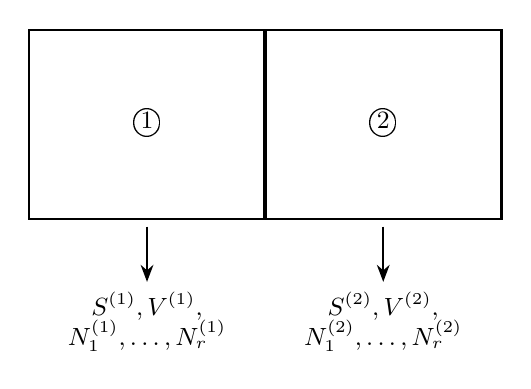
\begin{tikzpicture}
  \draw[caja] (0,0) rectangle (3,2.4);
  \draw[pared] (3,0) -- (3,2.4);
  \draw[caja] (3,0) rectangle (6,2.4);
  \node at (1.5,1.2) {\normalsize \textcircled{\small 1}};
  \node at (4.5,1.2) {\normalsize \textcircled{\small 2}};
  \draw[->,line width=0.7pt] (1.5,-0.1) -- (1.5,-0.8) node[below,align=center] {$S^{(1)},V^{(1)},$\\$N_1^{(1)},\dots,N_r^{(1)}$};
  \draw[->,line width=0.7pt] (4.5,-0.1) -- (4.5,-0.8) node[below,align=center] {$S^{(2)},V^{(2)},$\\$N_1^{(2)},\dots,N_r^{(2)}$};
\end{tikzpicture}
\end{document}
